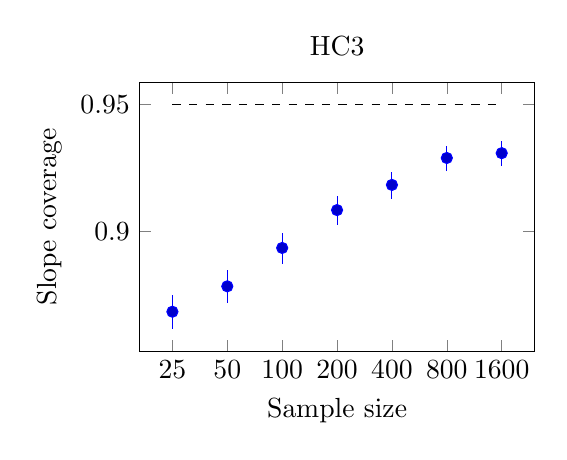
\begin{tikzpicture}
\begin{axis}[width=6.6cm,height=5cm,xlabel={Sample size},ylabel={Slope coverage},title={HC3},xtick={0,1,2,3,4,5,6},xticklabels={{25},{50},{100},{200},{400},{800},{1600}}]
% Interval meaning: Wilson 95% interval for coverage over 10000 trials
\addplot+[no marks,forget plot] coordinates {(0,0.8617346296685646) (0,0.8749823635322467)};
\addplot+[no marks,forget plot] coordinates {(1,0.8719508884456331) (1,0.8847584247877647)};
\addplot+[no marks,forget plot] coordinates {(2,0.8874046014402782) (2,0.899493115042325)};
\addplot+[no marks,forget plot] coordinates {(3,0.9026910992750709) (3,0.9139951740560862)};
\addplot+[no marks,forget plot] coordinates {(4,0.9128724734222167) (4,0.923606196741201)};
\addplot+[no marks,forget plot] coordinates {(5,0.9237998614131585) (5,0.9338706679848011)};
\addplot+[no marks,forget plot] coordinates {(6,0.9257617947322282) (6,0.9357072754719226)};
\addplot+[only marks,forget plot] coordinates {(0,0.8685) (1,0.8785) (2,0.8936) (3,0.9085) (4,0.9184) (5,0.929) (6,0.9309)};
\addplot[black,dashed,no marks,forget plot] coordinates {(0,0.95) (6,0.95)};
\end{axis}
\end{tikzpicture}
